\documentclass[12pt]{article}
\usepackage[utf8]{inputenc}
\usepackage{booktabs}
\usepackage{multicol}
\usepackage{graphicx}
\usepackage{fancyhdr}
\usepackage{lipsum}
\usepackage[style=numeric-comp]{biblatex}
\addbibresource{bibliography.bib}
\setlength{\columnsep}{4cm} %a djust base on your name length

\begin{document}
\pagenumbering{gobble}

%% Copertina
%!TEX encoding = UTF-8 Unicode
%!TEX root = thesisCASes.tex

\begin{center}

\includegraphics[width=12cm]{figures/logo-CSC-pdf-cropped.pdf} \\
\vspace{1cm}

%{\LARGE \textbf{Conservatorio di Musica Santa Cecilia}} \\
%\vspace{0.2cm}
{\Large {Dipartimento di Nuove Tecnologie e Linguaggi
Musicali}} \\ 
%\vspace{1cm}


%{\Large {Tesi di Laurea Biennale in Musica Elettronica}} \\
{\Large {Biennio Superiore di II Livello in Musica Elettronica}} \\[2.5cm]

{\Large {Tesi di Laurea}} \\[0.5cm]

{\LARGE \textbf{Sistemi Complessi Adattivi per la performance musicale in Live Electronics}} \\[2cm]

\end{center}

\begin{multicols}{2}
\noindent \large{Relatore:} \\
\large{\textbf{Giuseppe Silvi}} \\
\vspace{0.1cm}

\noindent {\large {Correlatori:}} \\
\large{\textbf{Agostino Di Scipio}} \\
\large{\textbf{Dario Sanfilippo}} \\
\vspace{0.1cm}

%% \noindent {\large {Controrelatore:}} \\
%% \large{\textbf{Prof. Name}} \\
%% \vspace{0.1cm}
\columnbreak

\noindent{\large {Candidato:}} \\
\large{\textbf{Luca Spanedda}} \\
\end{multicols}

\vfill

\begin{center}
    \large{\textbf{Anno Accademico 2021/2022}}
\end{center}
\newpage
\ 
\newpage

%% Dichiarazione di intenti
\vfill
\LARGE \textbf{Dichiarazione} \normalsize \newline \newline
Dichiaro che il sottoscritto nonché autore del
documento è il responsabile del suo contenuto, 
e per le parti tratte da altri lavori, 
queste vengono espressamente dichiarate
citando le fonti.
\
\newline
Luca Spanedda.
\ 
\newpage

%% Ringraziamenti
\vfill
\LARGE \textbf{Ringraziamenti} \normalsize \newline \newline
qui i ringraziamenti.
\newpage
\
\newpage

%% Abstract
\begin{abstract}
Il lavoro presentato qui è uno studio di implementazione, analisi ed esecuzione
di tre Sistemi Complessi Adattivi (CASs: Complex Adaptive Systems) 
creati appositiamente per la performance musicale (in Live Electronics),
la scelta di questi tre sistemi corrisponde a tre diversi casi di studio 
(case study) nell'implementazione di dinamiche nonlineari sfruttate 
per la generazione dei comportamenti emergenti nei Sisitemi Complessi.
Una prima parte del lavoro tratterà dell'implementazione e l'analisi di due brani,
creati rispettivamente da due compositori e ricercatori riconosciuti 
nell'ambito internazionale della Computer Music: Agostino Di Scipio e Dario Sanfilippo.
Di Agostino di Scipio studieremo un sistema con nonlinearità provenenti dal dominio analogico, 
che sfrutta fenomeni generativi nel mondo fisico riportati all'interno del sistema 
grazie alle conversioni AD/DA (analogico a digitale e viceversa). 
Di Dario Sanfilippo studieremo invece un sistema che sfrutta nonlinearità 
appositamente programmate dal compositore nel mondo digitale DSP (Digital Signal Processing),
tramite alcuni principi di autoregolazione, 
senza interazioni e perturbazioni provenienti dal mondo esterno. 
Infine la seconda parte del lavoro tratta l'implementazione di un mio brano,
ibrido fra i due casi di studio presentati qui,
che andrà a conclusione del lavoro di ricerca, analisi ed implementazione
svolto durante il corso della tesi.
\end{abstract}
\newpage
\

% conteggio pagine
\pagenumbering{arabic}

\tableofcontents
\listoftables
\listoffigures
\newpage

\pagestyle{fancy}


%% --------------------------------------------------- Capitoli ----------------
%% capitolo TEST
%%\input{chapters/0_TEST}

%% TITOLO
\section{Introduzione}
\label{sec:Introduzione}

%% TESTO
Dopo la crisi del sistema tonale (in uso in Occidente dal XVII secolo)
e dopo la crisi dei fondamenti delle scienze di inizio secolo,
le nascenti considerazioni strutturali e teoriche
nella musica alla ricerca di vie al di fuori del sistema tonale,
parallelamente all'esigenza di introdurre nuovi paradigmi all'interno delle scienze,
hanno contribuito all'avvenire di importanti punti di incontro fra i due ambiti.
\\
Uno dei più importanti avanzamenti nelle scienze
al termine della seconda guerra mondiale, risedette nell'introduzione della
cibernetica e della teoria generale dei sistemi, che hanno conseguentemente
portato alla nascita del pensiero sistemico e del concetto di scienze della complessità.
\\
La cibernetica in particolare ebbe inizio durante gli anni della seconda guerra mondiale e si deve al fisico e matematico Norbert Weiner.
Nel 1940 Wiener insieme ad altre ad altre prominenti figure provenienti da diversi ambiti scientifici,
come Ross Ashby, Margaret Mead, Gregory Bateson, Heinz von Foerster, partecipano ad una serie di conferenze
multidisciplinari chiamate "The Macy Conferences", inizialmente intitolate
"Feedback Mechanism in Biology and the Social Sciences" con l'obiettivo comune di andare a definire
gli ambiti di interesse della nuova scienza.
Il concetto sviluppato dai greci - kybernetes -
viene poi ripreso da Norbert Weiner nel 1948,
che ispirato dalla meccanica ed i suoi risultati durante la guerra
e contemporaneamente dallo sviluppo della teoria della comunicazione (o informazione) di Claude Shannon,
con la volontà di sviluppare una teoria generalizzata dei principi di
organizzazione e controllo nei sistemi emersi durante le conferenze pubblicherà un libro nel 1948:
La cibernetica, controllo e comunicazione nell'animale e nella macchina,
in cui definiva l'ambito di interesse e gli obiettivi della nuova disciplina,
inaugurando anche l'uso del nuovo termine da lui coniato; a seguito di questo libro che riscuoterà
un importante successo, le conferenze presero il nome di
"Cybernetics, Circular Causal, and Feedback Mechanism in Biological and Social Systems",
innalzando Wiener come la principale figura di spicco.
\\
La cibernetica è la scienza che studia i principi astratti di organizzazione
nei sistemi complessi.
In particolare come evidenziato fino ad ora dalla sua natura multidisciplinare,
non si interessa con particolare attenzione in cosa consistano questi sistemi,
quanto al più al loro funzionamento:
\\
- come usano l'informazione e come la scambiano gli agenti
\\
- come collaborano fra loro in direzione di un obiettivo comune
\\
- come contrastano il rumore
\\
e così via...
\\
Le fortunate premesse iniziali della cibernetica risiedevano in una convinzione
da parte di questi scienziati provenienti dai differenti ambiti disciplinari, che esistesse uno
"schema processuale" comune ad organismi viventi e macchine, rintracciato attraverso una ricerca uniforme garantita da dell'utilizzo di un metodo "sintetico" e "comportamentale".
Fra gli anni '60 e la metà del '70 la cibernetica grazie agli scienziati
Heinz von Foerster, Margaret Mead, e altri,
compierà un ulteriore passo fondamentale che la porterà
verso il compimento della stessa in una scienza concreta, divenendo la "Cibernetica di secondo ordine",
anche chiamata come "la cibernetica dei sistemi di osservazione", che consiste nell'applicazione
ricorsiva della cibernetica a se stessa e la pratica riflessiva della cibernetica
secondo tale critica.
La differenza fra cibernetica di primo e secondo ordine risiese nel fatto,
che mentre nel primo periodo lo studioso di cibernetica (di primo ordine)
studiava un sistema da un punto di vista passivo, da quello dell'osservatore
dei comportamenti di un sistema.
Il  cibernetico di secondo ordine lavora ed interviene nel comportamento
e nella costruzione di un sistema complesso,
riconoscendo il sistema come un agente con cui interagire e
riconoscendo esso stesso come agente nell'interazione col sistema.
\\
A partire dalle sue importanti premesse,
la cibernetica ha conseguentemente poi avuto un ruolo centrale nello sviluppo di
molti studi scientifici e la nascita
di nuovi ambiti come: l'intelligenza artificiale, la teoria del caos,
la teoria della catastrofe,
la teoria dei controlli, la teoria generale dei sistemi, la robotica,
la psicologia e le scienze sociali,
ecc.
nella mappa di B.Castellani e L.Gerrits riportata per intero nella pagina seguente,
possiamo visualizzare con più precisione e accurtezza
l'insorgere e l'evoluzione di questi paradigmi scientifici, per averne una
visione più completa relativa al loro sviluppo.

\clearpage

\begin{figure}[!h]
    \centering
    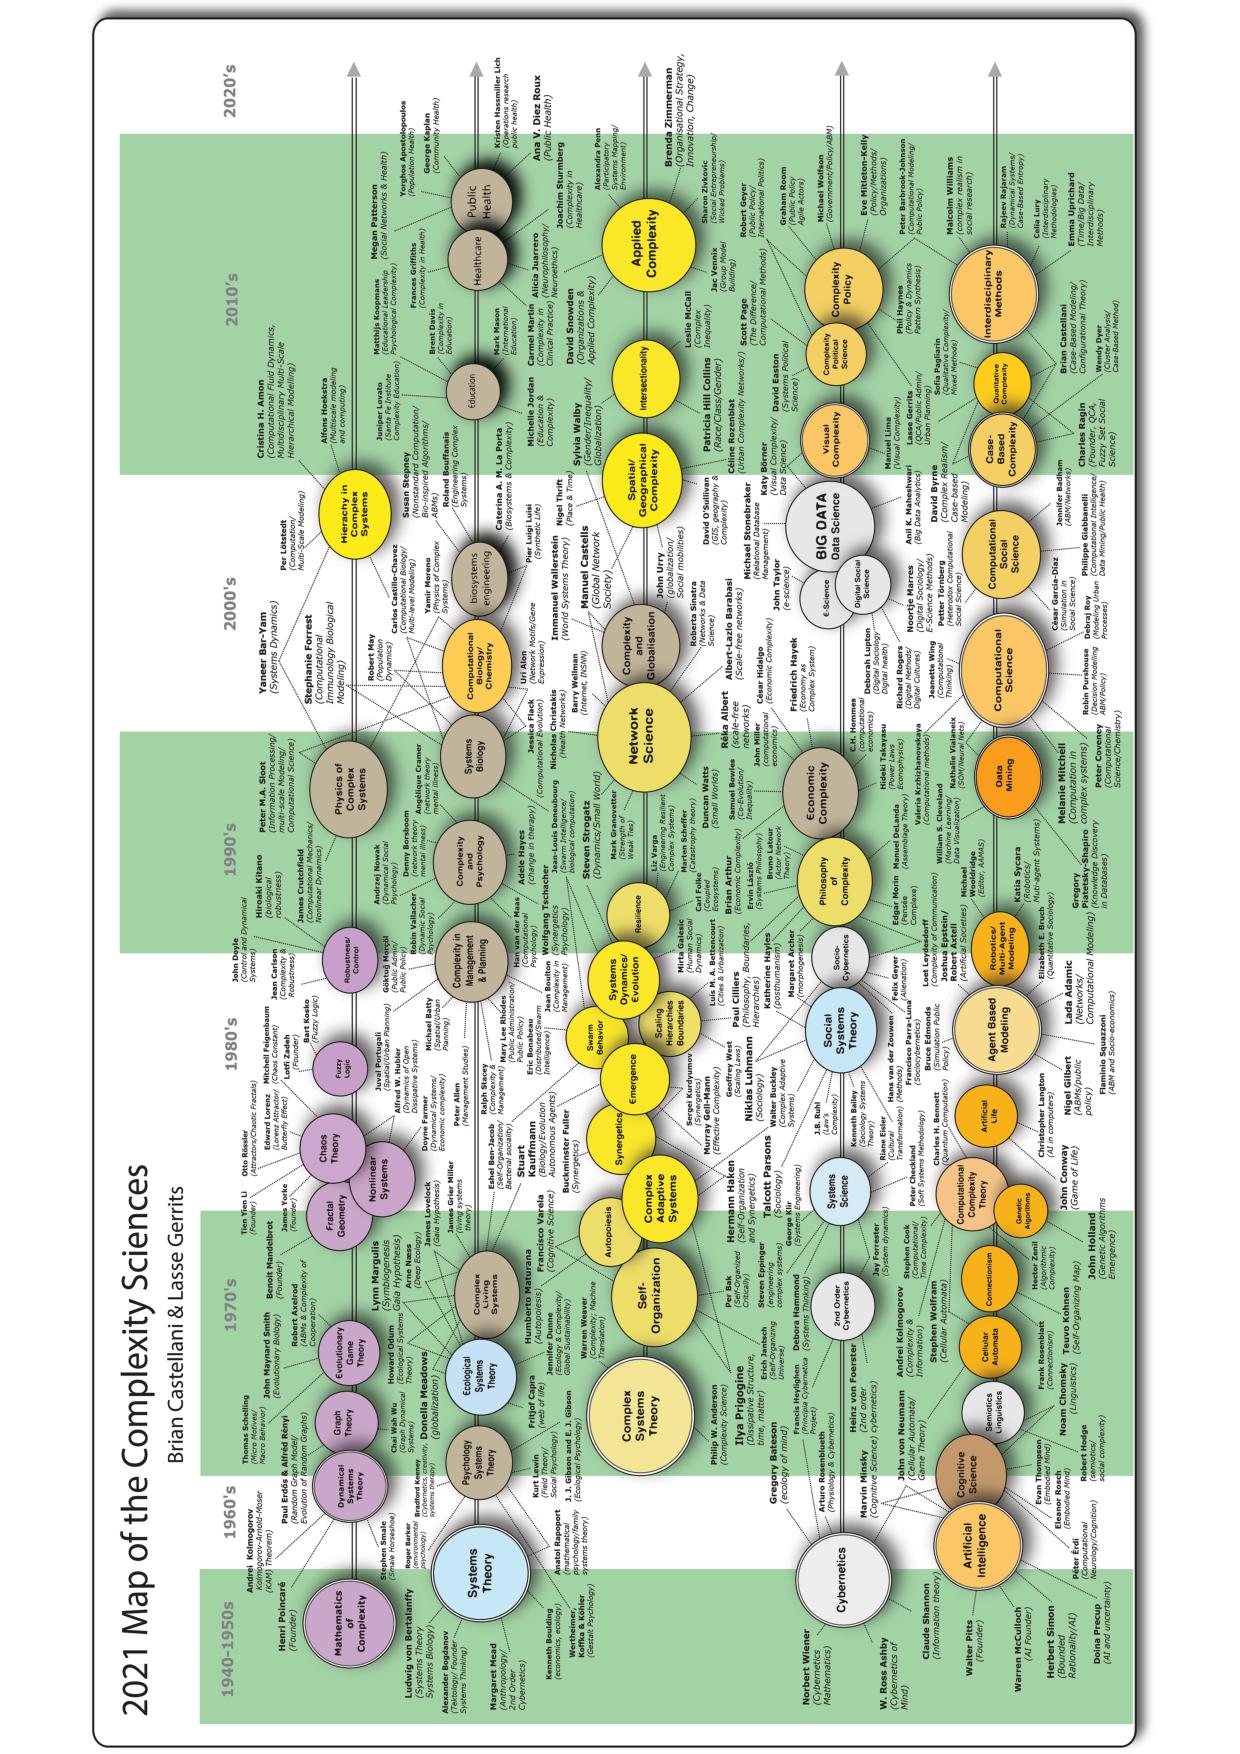
\includegraphics[width=1.0\textwidth, angle=0]{figures/complexitymap.pdf}
    \label{fig:figure}
\end{figure}
%% https://www.art-sciencefactory.com/MapLegend.html

\clearpage

\subsection{Le cibernetiche nella musica}
\label{sec:Le cibernetiche nella musica}
All'inizio degli anni '60 in seno alle nascita delle scienze complesse,
l'uso di sistemi di feedback e la rilevanza dei circuiti informativi chiusi
nelle strutture organizzate,
ha goduto di uno slancio popolare anche nel mondo della musica e più in generale dell'arte.
Uno dei primi nella storia dell'arte ad evocare l'uso della cibernetica nei propri lavori è stato
Nicolas Schoeffer con il suo ciclo di lavori "spazio-dinamici", in particolare ha creato
la prima installazione ad implementare meccanismi di auto-regolazione, il CYSP-1,
capace di essere sensibile all'ambiente esterno e a se stesso
grazie ad una serie di tecnologie offerte dalla compagnia Philips (fotocellule e microfoni),
e reagire sonoramente a questi stimoli riproducendo
una serie di registrazioni composte dal compositore francese Pierre Henry,
collaboratore di Pierre Schaeffer ed insieme a lui figura centrale nella nascita della Musique concrète.
Un'altra importante esperienza del periodo iniziale è quella del compositore Roland Kayn,
che dopo essersi avvicinato alla musica elettronica sotto la guida di Herbert Eimert
nello studio di Colonia (1954),
e dopo essersi trasferito a Roma nel 1960, dal 1964 assieme ad Aldo Clementi e Franco Evangelisti
fonda il Gruppo di improvvisazione Nuova Consonanza, del quale fece parte sino al 1968,
ed in quel periodo ispirato dalle teorie della cibernetica iniziò a sperimentare
estensivamente con sistemi di autoregolazione basati su feedback loops,
sia come modelli formali per composizioni strumentali che come reti di generatori di segnale analogici.
Tuttavia, a parte casi popolari di deliberate dichiarazioni formali da parte degli artisti,
come è nel caso di Roland Kayn,
non bisogna pensare a questi lavori appena citati (ed altri riportati a seguito),
come ad atti pioneristici che sancisono la nascita della cibernetica in musica,
ma proprio come si dice per la scoperta del fuoco
lo scenario più accurato risiede probabilmente nel fatto che
tanti autori provenienti da diverse parti del mondo, nello stesso periodo
sono stati influenzati e si sono influenzati a vicenda con le stesse idee
provenienti da un interesse condiviso per le teorie cibernetiche di Weiner e delle Macy Conferences.
Si può pensare ad esempio a quelle che sono le esperienze dello studio di Colonia:
nel 1951, Herbert Eimert e Werner Meyer-Eppler persuasero il direttore della NWDR, Hanns Hartmann,
a creare uno Studio per la Musica Elettronica, che Eimert diresse fino al 1962.
Questo è diventato lo studio più influente al mondo durante gli anni 1950 e 1960,
con ospiti alcuni dei più importanti compositori contemporanei provenienti da tutta europa,
come il già citato Roland Kayn, Franco Evangelisti, Karlheinz Stockhausen, Herbert Brun,
Cornelius Cardew, e molti altri.
Qui è dove nel 1964 K.Stockhausen lavora a "Mikrophonie I", che seppure non dichiarato è un ovvio punto di inizio
se si pensa a quelle logiche di interazione sistemiche fra uomo/macchina/ambiente in musica,
e in quel caso un punto di formalizzazione importante per quella che sarà l'esperienza del live electronics,
e non a caso in quel periodo il lavoro di ricerca condotto da Werner-Meyer Eppler,
scienziato, musicista ideatore e direttore dello studio di Colonia,
ha trovato sin dalla nascita dello studio fondamento in quelle che sono state
le teorizzazioni della Cibernetica.
Parlando sempre dello studio di colonia, c'è poi il caso di Franco Evangelisti,
come citato prima fondatore insieme a Roland Kayn del Gruppo Improvvisazione Nuova Consonanza,
che in quel periodo (qualche anno prima della fondazione del Gruppo a Roma)
si trova nello studio di Colonia per lavorare al brano "Incontri di Fasce Sonore",
e quando farà ritorno a Roma poi citerà più volte deliberatamente in interviste, scritti,
e altre documentazioni, il suo approccio sistemico/cibernetico a quelle che saranno le esperienze con
Gruppo.
O ancora, se cambiamo paese e passiamo dall'Europa od osservare l'America in quel periodo,
possiamo pensare a quelli che sono i lavori di Louis e Bebe Barron,
con i circuiti in retroazione destinati al corto circuito
e utilizzati appositamente come materiale per la generazione acustica di trame incise su nastro,
o ai lavori di John Cage come "Electronic Music for piano" o di Steve Reich come "Pendulum Music" del 1968,
che sfruttano ed esplorano l'effetto Larsen in modo artistico.
\\
Un secondo periodo costituito da un approccio sistemico più consapevole
che inizia a tracciare la strada per un pensiero ecosistemico della composizione, inizia dal lavoro
di Alvin Lucier, che nel 1969 scriverà quello che sarà un brano emblematico per
la cibernetica in musica "I'm sitting in a room", altro brano importante per quelle che sono
le logiche di interazione sistemiche fra uomo/macchina/ambiente e che sancisce una volta per tutte
l'interazione sistemica dove il musicista l'ambiente e lo strumento sono parti di un insieme del
sistema "più complesso" con un comportamento collettivo derivato dai singoli agenti,
in un un'interazione con l'ambiente circostante.
In I'm sitting in a room, un performer al centro della stanza
recita in un microfono un testo che descrive il fenomeno che avverrà poco a poco,
la voce recitante nel microfono viene registrata e poi riprodotta da altoparlanti
posti nella stanza, il suono della regitrazione riprodotta da questi altoparlanti
viene registrato nuovamente durante la riproduzione, l'operazione
viene ripetuta in un in una casualità circolare di volta in volta dove alla fine rimarranno
solo i contributi provenienti dalla stanza, dalla voce e dalla catena elettroacustica,
dando vita nel loro insieme ad un effetto Larsen, la natura
nonlineare del processo e degli agenti porterà di volta in volta ad un risutato
sempre differente.
Dopo l'esperienza di Lucier, nel 1974 Nicolas Collins compone "pea soup"
mentre è studente alla Wesleyan University.
Pea soup consiste in una rete adattiva di circuiti analogici (3 Countryman Phase Shifters),
che intona il feedback positivo dell'effetto Larsen ad una frequenza risonante diversa
ogni volta che questo inzia ad emergere.
Ad oggi svariati compositori a partire dalle trame delineate dalle scienze complesse e
dai lavori citati operano nell'ambito della musica elettronica con un approccio sistemico,
un importante caso è quello di Agostino Di Scipio, che contribuisce significatamente
nell'ambito della computer music sin dai primi anni '90, divenendo una
delle figure più importanti nell'area della composizione ecosistemica e nel suo
caso in particolare del live electronics, o quello di Dario Sanfilippo
compositore e ricercatore con all'attivo recenti importanti pubblicazioni e lavori
nell'ambito dei sistemi di feedback in musica, e in particolare di non linearità nei sistemi
in DSP.


\printbibliography
\appendix 
\section{Primo appendice}

In questo appendice sono riportati tutti i codici dei sistemi
e le relative librerie di oggetti trattati nel corso della tesi. \\
\verb| Audible_Ecosystemics_2.dsp | è il file principale di una implementazione 
completa del sistema di Audible Ecosystemics 2 di Agostino Di Scipio, sviluppato con il supporto
e il prezioso aiuto di Dario Sanfilippo, nel Debug del sistema e sviluppo della libreria del codice; 
e conseguente al prezioso lavoro svolto con i miei compagni nella Classe di esecuzione ed interpretazione 
della musica elettroacustica di Giuseppe Silvi, che mi ha permesso di approfondire le tematiche
discusse nel corso della tesi riguardo al brano e poter sviluppare strategie efficaci per questa implementazione.
\verb| aelibrary.lib | è invece la libreria degli oggetti utilizzati nella implementazione del sistema
di Audible Ecosystemics 2 di Agostino Di Scipio (oggetti discussi anche nella tesi). \\
\verb| RITI_v1_CelloC2.dsp | è il file principale della implementazione 
del mio sistema di RITI v.1.0. \verb| RITI.lib | è invece la libreria degli oggetti utilizzati nella 
implementazione del mio sistema di RITI v.1.0. \verb| SpectreLists.lib | è infine una libreria
con i risultati delle analisi condotte sulle note del violoncello, utilizzata per passare le informazioni
ai filtri passabanda nel sistema di RITI v.1.0. \\
\clearpage


\begin{center} \Large \verb| Audible_Ecosystemics_2.dsp | \normalsize \\
    \vspace{0.2cm} \end{center}
\lstinputlisting[breaklines, frame=trBL]{codes/Audible_Ecosystemics_2.dsp}
\clearpage

\begin{center} \Large \verb| aelibrary.lib | \normalsize \\
    \vspace{0.2cm} \end{center}
\lstinputlisting[breaklines, frame=trBL]{codes/aelibrary.lib}
\clearpage

\begin{center} \Large \verb| RITI_v1_CelloC2.dsp | \normalsize \\
    \vspace{0.2cm} \end{center}
\lstinputlisting[breaklines, frame=trBL]{codes/RITI_v1_CelloC2.dsp}
\clearpage

\begin{center} \Large \verb| RITI.lib | \normalsize \\
    \vspace{0.2cm} \end{center}
\lstinputlisting[breaklines, frame=trBL]{codes/RITI.lib}
\clearpage

\begin{center} \Large \verb| SpectreLists.lib | \normalsize \\
    \vspace{0.2cm} \end{center}
\lstinputlisting[breaklines, frame=trBL]{codes/SpectreLists.lib}
\clearpage

\section{Secondo appendice}

In questo appendice sono riportati i codici utilizzati per le analisi 
spettrali del violoncello effettuati in Python per il sistema RITI v.1.0. \\
\verb| FFT_range.py | il primo prototipo di questo codice è stato sviluppato
in collaborazione con il mio collega e amico Edoardo Staffa. 
L'analisi DFT del file audio può essere effettuata scegliendo il numero di Bins e 
il Range in frequenza da analizzare (il Bandwidth è ricavato sulla base di questi dati),
l'output dell'analisi è sia un plot di uno spettrogramma in formato .html navigabile,
che un file di testo con tutti i dati: frequenze, ampiezze e Bandwidth.
\verb| sort_amplitudes.py | prende la lista generata ed effettua un sort
decrescente delle liste a partire dalle frequenze con i picchi di ampiezza più 
elevati a quelli meno elevati. \verb| filter_frequencies.py | elimina le frequenze 
dalle liste troppo vicine ai picchi più elevati (impostato di default a 40Hz).
\verb| sort_frequencies.py | effettua il sort per frequenze in ordine crescente.
\verb| makelib.py | infine converte le liste .txt processate in un file .lib leggibile da Faust.
\clearpage


\begin{center} \Large \verb| FFT_range.py | \normalsize \\
    \vspace{0.2cm} \end{center}
\lstinputlisting[breaklines, frame=trBL]{codes/FFT_range.py}
\clearpage

\begin{center} \Large \verb| sort_amplitudes.py | \normalsize \\
    \vspace{0.2cm} \end{center}
\lstinputlisting[breaklines, frame=trBL]{codes/sort_amplitudes.py}
\clearpage

\begin{center} \Large \verb| filter_frequencies.py | \normalsize \\
    \vspace{0.2cm} \end{center}
\lstinputlisting[breaklines, frame=trBL]{codes/filter_frequencies.py}
\clearpage

\begin{center} \Large \verb| sort_frequencies.py | \normalsize \\
    \vspace{0.2cm} \end{center}
\lstinputlisting[breaklines, frame=trBL]{codes/sort_frequencies.py}
\clearpage

\begin{center} \Large \verb| makelib.py | \normalsize \\
    \vspace{0.2cm} \end{center}
\lstinputlisting[breaklines, frame=trBL]{codes/makelib.py}
\clearpage


\end{document}